\documentclass{article}
\usepackage[utf8]{inputenc}
\usepackage{blindtext}
\usepackage{titlesec}
\usepackage{geometry}
\usepackage{listings}
\usepackage{graphicx}
\usepackage{amsfonts}
\usepackage{amssymb}
\usepackage{amsmath}
\usepackage{hyperref}
\usepackage{color}
\usepackage{float}
\usepackage{units}
\usepackage{mathtools}
\usepackage{soul}
\usepackage{enumitem}
\usepackage{siunitx}
\usepackage{multirow}
\usepackage[bottom]{footmisc}
\usepackage{minted}
\usepackage{mdframed}
\usepackage{caption}
\usepackage{xcolor}

\newlength\dlf
\newcommand\alignedbox[3][yellow]{
  % #1 = color (optional, defaults to yellow)
  % #2 = before alignment
  % #3 = after alignment
  &
  \begingroup
  \settowidth\dlf{$\displaystyle #2$}
  \addtolength\dlf{\fboxsep+\fboxrule}
  \hspace{-\dlf}
  \fcolorbox{red}{#1}{$\displaystyle #2 #3$}
  \endgroup
}

\newcommand{\highlight}[1]{%
  \colorbox{yellow!50}{$\displaystyle#1$}}
\newcommand{\highlightred}[1]{%
  \colorbox{red!50}{$\displaystyle#1$}}

\geometry{
 a4paper,
 total={170mm,257mm},
 left=20mm,
 top=20mm,
 }


\setlength{\parindent}{0pt}

\title{Digital Systems Design - Report 3}
\author{pranav.malhotra13 }
\date{March 2016}

\begin{document}

\begin{titlepage}
	\centering
	{\scshape\LARGE Imperial College London \par}
	\vspace{2cm}
	{\scshape\Large Digital Systems Design \par}
	\vspace{1cm}
	{\scshape\Large Report 3 \par}
	\vspace{2.5cm}
	{\Large\itshape Dada Oluwatomisin, CID: 0084614 \par}
	\vspace{1.0cm}
	{\Large\itshape Pranav Malhotra, CID: 00823617 \par}
	\vfill
	{\large \today\par}
\end{titlepage}

\tableofcontents
\newpage
%%%%%%%%%%%%%%%%%%%%%%%%%%%%%%%%%%%%%%%%%%%%INTRODUCTION%%%%%%%%%%%%%%%%%%%%%%%%%%%%%%%%%%%%%%%%%%%%%
\section{Introduction}
The task set out in the Digital Systems Design coursework is to accelerate the computation of the complex expression listed in equation (\ref{eq:complex_expression}).

\begin{align}
    f(x) = \sum_{i=1}^{N} 0.5x_{i} + x_{i}^{2}cos(floor\big(\frac{x_{i}}{4}\big)-32)\label{eq:complex_expression}
\end{align}


In the two previous reports multiple aspects of this task have been explored.\\ 
 
Firstly, an analytic approach to solving the problem was explored. Although this worked for previous elementary tasks, it is not applicable for more complex expressions, like equation (\ref{eq:complex_expression}), that do not have an analytical form. \textbf{Also, such an implementation strays away from the objectives and learning lessons set out in the coursework.} Secondly, brief error analysis was conducted. The error analysis provided some insight into the shortcomings of floating point numbers. Interfacing with external memories was introduced; this is necessary since it not possible to store all instructions and data near the cpu on on-chip memories. The overhead associated with fetching data/instructions was studied. It was discovered that the use of caches can significantly reduce the overall latency of the system. Analysis was then conducted to determine the ideal cache size. \textbf{A balanced approach would suggest using $8Kb$ of cache memory. However, the task requires accelerating the evaluation of the complex equation given all the resources on the Altera DE0 Board and thus a cache size of $32Kb$ was decided upon.} Lastly, dedicated hardware to implement fixed-point multiplication was added to the processor. This additional hardware had a sizable effect in accelerating the evaluation of the complex expression.\\

\textbf{The next step is to fully map the evaluation of the complex expression onto hardware.} This report will present multiple design considerations, learning lessons, as well as the final design. Error analysis will be conducted to evaluate the accuracy of the system. The trade-off between resource utilisation and achieved latency will be considered.

%%%%%%%%%%%%%%%%%%%%%%%%%%%%%%%%%%%%%CORRECTIONS FROM REPORT 2%%%%%%%%%%%%%%%%%%%%%%%%%%%%%%%%%%%%%%%%%%%%%
\section{Corrections from Report 2}
In report 2, table \ref{tab:report_2_erronous_table} was presented. 

\begin{table}[H]
  \centering
    \begin{tabular}{|c|c|c|c|c|}
    \hline
    \multirow{2}{*}{\textbf{N}} & \multirow{2}{*}{\textbf{Step}} & \textbf{MATLAB} & \textbf{{\tt generateVectorAddition}} & \textbf{{\tt generateVectorMultiplication}} \\
    \cline{4-5}          &       & \textbf{Result} & \textbf{Percentage Error} & \textbf{Percentage Error} \\
    \hline
    52    & 5     & 57880.00 & 0.0002\% & 0.0002\% \\
    \hline
    511   & 0.5   & 34026.00 & -0.0004\% & -0.0004\% \\
    \hline
    2551  & 0.1   & -68594.00 & -12.2159\% & -0.0022\% \\
    \hline
    25501 & 0.01  & -1223100.00 & -30.0492\% & 0.0024\% \\
    \hline
    255001 & 0.001 & -12768000.00 & 389.9631\% & 0.0034\% \\
    \hline
    \end{tabular}%
  \caption{Incorrect error analysis for task 4}
  \label{tab:report_2_erronous_table}
\end{table}%
  
The function {\tt generateVectorMultiplication} presented in listing \ref{lst:generateVectorMultiplication} was observed to produce a result with a smaller percentage error with respect to the reference value generated in MATLAB. This is however incorrect. \textbf{The reference value that the result was compared to was wrong; it was incorrectly generated on MATLAB.}

\begin{listing}[H]
\begin{minted}[fontsize=\scriptsize,linenos]{C}
void generateVectorMultiplication(float x[N]){
	int i;
	
	// initialise first element
	x[0]=0;
	
	// generating vector through multiplication
	for(i=1; i<N; i++)
		x[i]=i*step;
}
\end{minted}
\caption{{\tt generateVectorMultiplication}} 
\label{lst:generateVectorMultiplication}
\end{listing}


The most accurate way to obtain a reference value is to import the input vector generated on the NIOS II processor onto MATLAB, perform all calculations using double-precision floating point numbers and obtain a result. Calculated in such a way, the reference value, for test case 3, that results should be compared to is $37022686.6086$. Table \ref{tab:report_2_correct_table} presents the updated error analysis.


\begin{table}[H]
  \centering
    \begin{tabular}{|c|c|c|c|c|}
    \hline
    \multirow{2}{*}{\textbf{N}} & \multirow{2}{*}{\textbf{Step}} & \textbf{MATLAB} & \textbf{{\tt generateVectorAddition}} & \textbf{{\tt generateVectorMultiplication}} \\
    \cline{4-5}          &       & \textbf{Result} & \textbf{Percentage Error} & \textbf{Percentage Error} \\
    \hline
    52    & 5     & 57879.87 & -3.17E-06\% & -3.18E-06\% \\
    \hline
    511   & 0.5   & 34026.04 & 9.73E-05\% & 9.74E-05\% \\
    \hline
    2551  & 0.1   & -76972.25 & -1.04E-04\% & -10.88\% \\
    \hline
    25501 & 0.01  & -1590647.07 & -6.309E-05\% & -23.11\% \\
    \hline
    255001 & 0.001 & 37022686.60 & 3.085E-05\% & -134.49\% \\
    \hline
    \end{tabular}%
  \caption{Correct error analysis for task 4}
  \label{tab:report_2_correct_table}
\end{table}%


\textbf{This does not mean that the assertion made in the previous report, that the way that the input vector is generated introduces errors into the final value, is completely invalid.} The input vector generated on the NIOS II processor is not ideal. There are errors in the vector; the vector is stored as an array of single-precision floating point numbers and thus the precision of the numbers is limited especially since small and large numbers are summed when the vector is being generated. \textbf{This is a limitation of the single-precision floating point number system. That being said, no practical number system can fully represent all real numbers and thus a balanced trade-off between accuracy, memory requirements and latency has to be made.}\\ 

\textbf{For the task at hand, the input vector is an invariant. Thus, it is best to focus on the inaccuracies introduced into the system through the custom hardware rather than the input vector.} As such, all systems are tested with an input generated using the function {\tt generateVectorAddition} presented in listing \ref{lst:generateVectorAddition}.

\begin{listing}[H]
\begin{minted}[fontsize=\scriptsize,linenos]{C}
void generateVectorAddition(float x[N]){
	int i;
	
	// initialise first element
	x[0] = 0;
	
	// generating vector by accumulating result
	for(i=1; i<N; i++)
		x[i]=x[i-1]+step;
}
\end{minted}
\caption{{\tt generateVectorAddition}} 
\label{lst:generateVectorAddition}
\end{listing}


\newpage
%%%%%%%%%%%%%%%%%%%%%%%%%%%%%%%%%%%%%TASK 6%%%%%%%%%%%%%%%%%%%%%%%%%%%%%%%%%%%%%%%%%%%%%
\section{Task 6: Floating Point Units through Custom Instructions}

In task 5, dedicated hardware capable of performing fixed-point multiplications was added. Two different approaches were considered; logic elements and embedded multipliers. Embedded multipliers proved more efficient at accelerating the evaluation of the function. \textbf{However, both logic elements and embedded multipliers only provide support for fixed-point multiplication.} Floating point multiplication is a much more involved process.\\ 

The steps for floating point multiplication are:
\begin{itemize}
    \item Add the exponents to find the new exponents. 
    \item Adding biased exponents causes the bias to be doubled. This has to be accounted for by subtracting the additional bias.
    \item Multiply the mantissas together.
    \item Normalise the result.
    \item Perform rounding.
\end{itemize}

\textbf{Adding embedded multipliers only provides dedicated hardware for the multiplication step. The other steps still need to be emulated in software. It would be ideal to perform the entire floating point multiplication process in hardware.} This requires the use of custom instructions on the Altera DE0 Board. Three types of custom instructions can be implemented on the Altera DE0 board. They are:
\begin{itemize}
    \item Combinational: Single clock cycle custom logic blocks.
    \item Multicycle: Multi-clock cycle custom logic blocks of fixed or variable durations.
    \item Extended: Custom logic blocks that are capable of performing multiple operations
\end{itemize}

\subsection{Design Considerations}\label{sec:design_considerations}
Before a custom instruction type is chosen and dedicated hardware is introduced, a set of design considerations needs to be formulated. 

\begin{enumerate}
    \item \textbf{The design should allow as many operations as possible to be performed on custom hardware.} As discussed above, any floating-point operation not performed on dedicated hardware will be emulated on software. This is not ideal as software emulation is costly. As such, the design should be capable of performing both floating-point additions and floating-point multiplications; both additions and multiplications are necessary to evaluate equation (\ref{eq:complex_expression}).
    \item \textbf{The design should be implemented such that the number of custom instruction calls is minimised.} The custom hardware should aim to reduce the number of iterations of the {\tt for} loop, needed to run through the entire input vector. This would be possible if the custom hardware is capable of processing more than one element in the input vector during each custom instruction call.
    \item \textbf{The hardware should return a result as soon as possible.} There should not be unnecessary delays within the custom hardware block.
    \item \textbf{The design should minimise the amount of resources used.} However, should there be a scenario where resources can be traded to reduce the latency, the design which reduces the latency will be preferred. 
\end{enumerate}

\subsection{Choosing Custom Instruction Type}
It is clear that extended would provide the greatest flexibility in terms of offloading multiple operations from the cpu onto the custom hardware. In addition, extended requires a \textbf{\textit{done}} signal to be asserted once the result is ready. The \textbf{\textit{done}} signal can be used to optimise a system in which different operations have a different latencies. Finally, extended takes two data inputs. The two inputs can be utilised to optimise the system, either by performing multiple calculations in parallel or by pipelining the system and performing multiple calculations sequentially.\\
\newpage
The timing diagram for the extended custom instruction is provided in figure \ref{fig:extended_custom_timing}.

\begin{figure}[H]
    \centering
    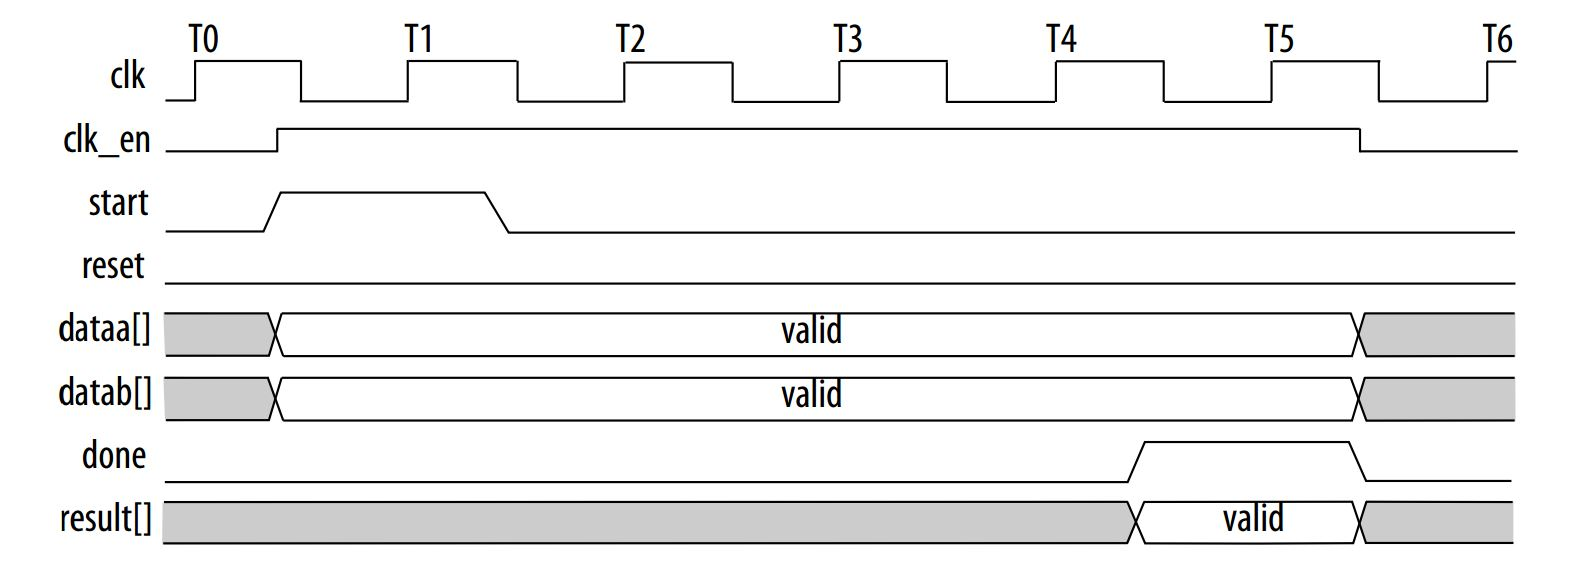
\includegraphics[width=0.99\textwidth]{extended_custom_instruction}  
    \caption{Timing diagram for extended custom instruction}
    \label{fig:extended_custom_timing}
\end{figure}

\subsection{Implemented Design}\label{sec:implemented_design}
Based on design consideration $1$, as many floating-point operations as possible should be mapped onto custom hardware. The custom instruction is designed to support both floating-point additions and floating point multiplications. Figure \ref{fig:task6_bdf_1} shows the schematic of the design. Two inbuilt Altera IP blocks, namely {\tt ALTFP\_ADD\_SUB} and {\tt ALTFP\_MULT} are used. A 1-bit select signal named \textbf{\textit{sel}} is incorporated into the design. 

\begin{figure}[H]
    \centering
    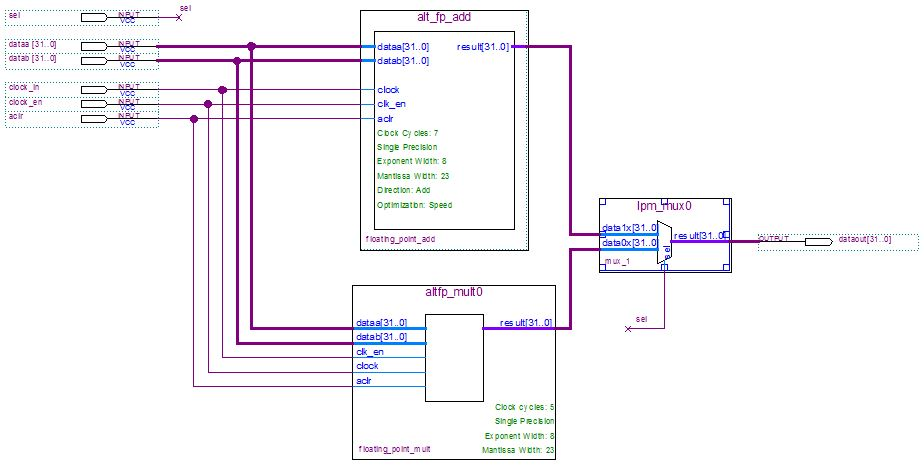
\includegraphics[width=0.99\textwidth]{task6_bdf_1}
    \caption{Task 6 design}
    \label{fig:task6_bdf_1}
\end{figure}

Table \ref{tab:task6} details the operation that is performed with respect to the select signal. 

\begin{table}[H]
  \centering
    \begin{tabular}{|c|c|}
    \hline
    \multicolumn{2}{|c|}{\textbf{Extended Custom Instruction}}\\
    \hline
    \textbf{sel} & \textbf{Operation Performed} \\
    \hline
    0    & Multiplication \\
    \hline
    1    & Addition \\
    \hline
    \end{tabular}%
  \caption{Operations corresponding to \textbf{\textit{select}} signal}
  \label{tab:task6}%
\end{table}%

\textbf{It is important to note that both addition and multiplication are performed at the same time. The correct output is selected through the use of a multiplexer.} Based on design consideration $3$, it is important that there is no unnecessary delay within the system. The two Altera IP blocks that are used have different latencies. Floating-point addition has a latency of $7$ clock cycles whereas floating-point multiplication has a latency of $5$ clock cycles. As such, it is important to assert the done signal at the appropriate time, based on the instruction that is being performed. Figure \ref{fig:task6_bdf_2} shows the schematic of the hardware that generates the \textbf{\textit{done}} signal.

\begin{figure}[H]
    \centering
    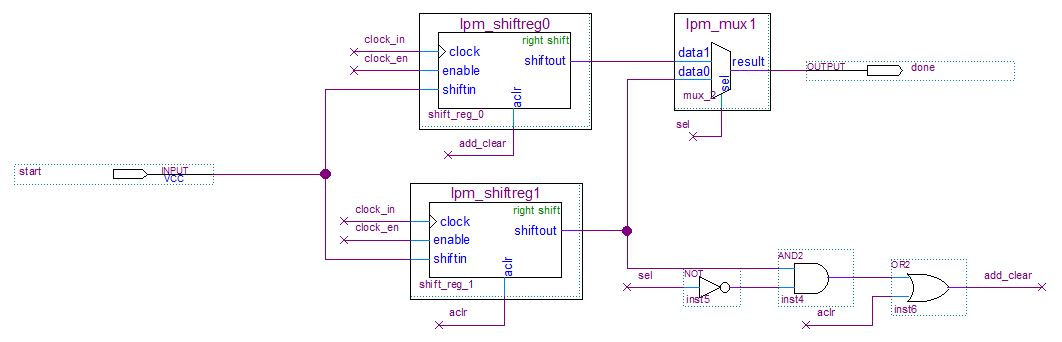
\includegraphics[width=0.8\textwidth]{task6_bdf_2}
    \caption{Task 6 \textbf{\textit{done}} signal generator}
    \label{fig:task6_bdf_2}
\end{figure}


\subsection{Results for Task 6}

\subsubsection{Evaluation of Function on NIOS II Processor}\label{sec:task6_nios_code}
Listing \ref{lst:task6_NIOS_code} presents the function {\tt sumVector\_FP\_ARTHEMETIC\_SUPPORT} that makes use of the custom instruction designed in section \ref{sec:implemented_design} to offload floating-point arithmetic to custom hardware. 

\begin{listing}[H]
\begin{minted}[fontsize=\scriptsize,linenos]{C}
// function performs operations in such a way so as to minimise custom instruction calls
float sumVector_FP_ARTHEMETIC_SUPPORT(float x[], int M){

	int i;
	// variable to hold final sum
	float running_sum = 0;
	
	// variable to hold value of complex expression for 1 input
	float current_value = 0;
	
	// number of iterations is equal to length of the vector
	for(i=0; i<M; i++){
		
		// evaluate cosine using math.h library
		current_value = cos(floor(x[i]/4)-32);
		
		// performs multiplication
		// xcos(floor(x/4)-32)
		current_value = ALT_CI_FP_ARITHMETRIC_SUPPORT_0(0, x[i], current_value);
		
		// adds half to current sum
		// 0.5 + xcos(floor(x/4)-32)
		current_value = ALT_CI_FP_ARITHMETRIC_SUPPORT_0(1, 0.5, current_value);
		
		// multiplies by number
		// x(0.5 + xcos(floor(x/4)-32))
		current_value = ALT_CI_FP_ARITHMETRIC_SUPPORT_0(0, x[i], current_value);

		// updates running sum
		running_sum = ALT_CI_FP_ARITHMETRIC_SUPPORT_0(1, running_sum, current_value);
	}
	
	// returns running_sum
	return running_sum;
}
\end{minted}
\caption{{\tt sumVector\_FP\_ARTHEMETIC\_SUPPORT}} 
\label{lst:task6_NIOS_code}
\end{listing}



The evaluation of the equation has been broken down into multiple stages. This allows all floating-point arithmetic to be performed using the custom hardware while minimising the number of function calls. \textbf{Having a design that minimises custom instruction calls is design consideration $2$; for task 6, this has been achieved by smart evaluation of the equation in software rather than by adding additional hardware support to deal with two inputs at the same time.}

\subsubsection{Comparison of Latency}\label{sec:compare_latency_6}
The latency of the system designed in section \ref{sec:implemented_design} is compared to the latency of the system designed for task 5. \textbf{In task 5, floating-point arithmetic was emulated in software and thus adding the custom instruction should greatly reduce the latency of the system.} Table \ref{tab:task6_latency} compares the latency achieved in task 5 to the latency achieved in task 6. Figure \ref{fig:task6_latency_graph} presents the same data graphically.


\begin{table}[H]
  \centering
    \begin{tabular}{|c|c|c|c|}
    \hline
    \textbf{N} & \textbf{Step} & \textbf{Task 5 (ticks)} & \textbf{Task 6 (ticks)} \\
    \hline
    52    & 5     & 19    & 16 \\
    \hline
    511   & 0.5   & 185   & 164 \\
    \hline
    2551  & 0.1   & 927   & 820 \\
    \hline
    25501 & 0.01  & 9259  & 8182 \\
    \hline
    255001 & 0.001 & 92801 & 82010 \\
    \hline
    \end{tabular}%
  \caption{Comparison of latency improvement}
  \label{tab:task6_latency}%
\end{table}%


\begin{figure}[H]
    \centering
    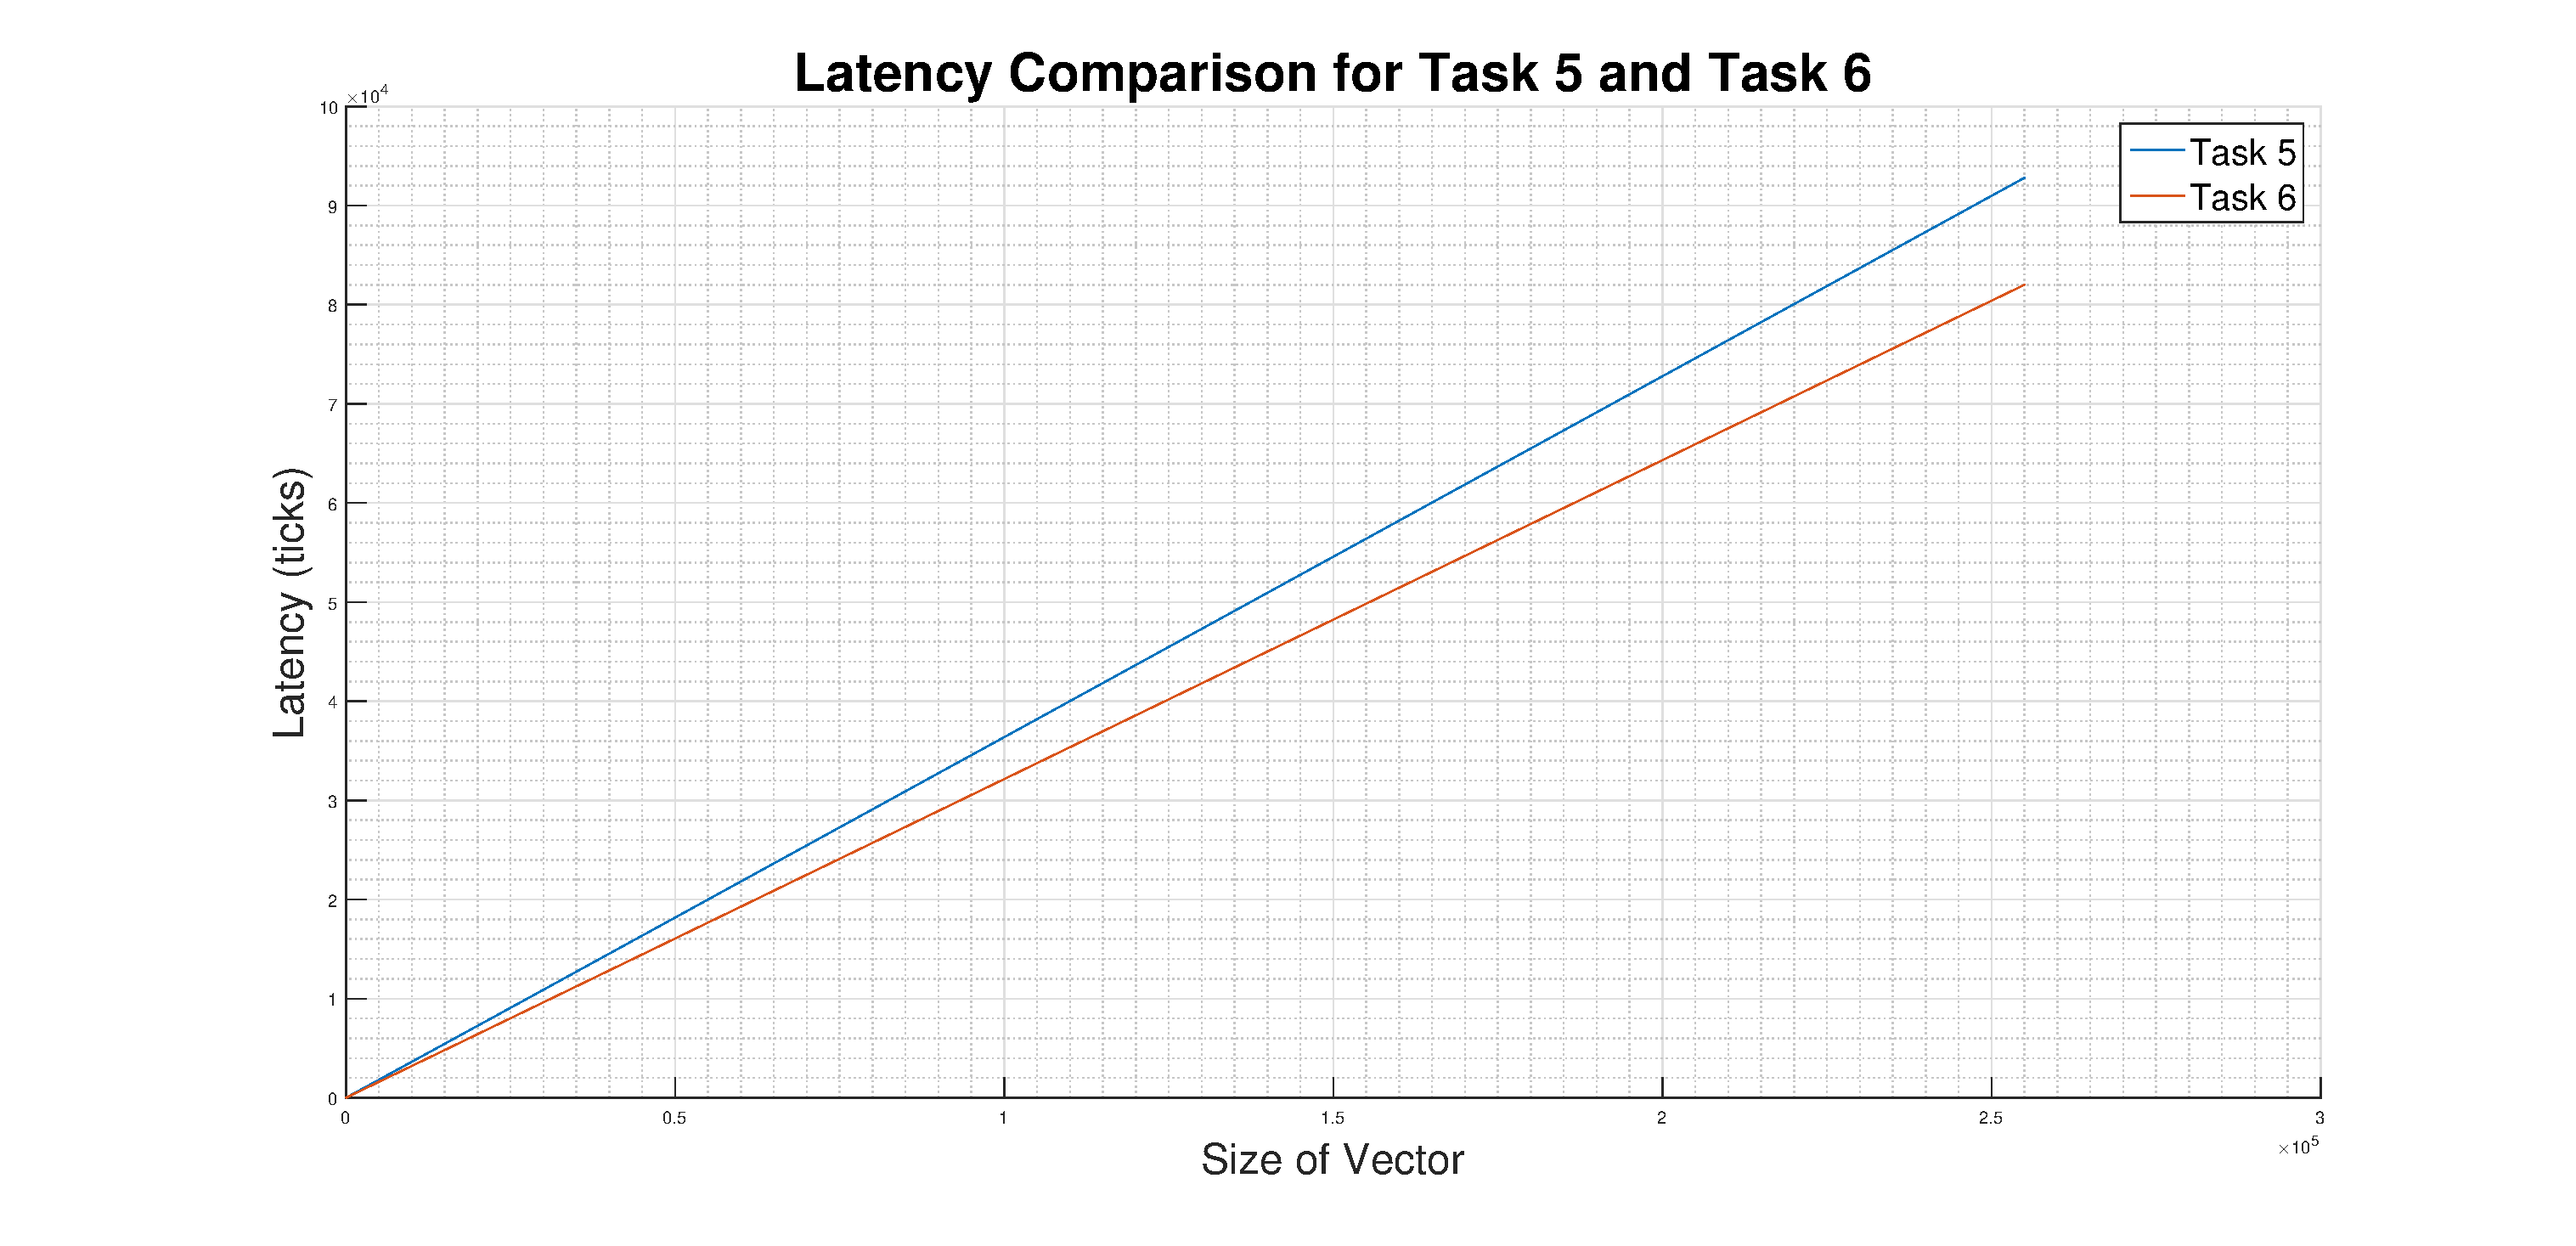
\includegraphics[width=0.7\textwidth]{task_6_latency}
    \caption{Comparison of latency improvement}
    \label{fig:task6_latency_graph}
\end{figure}

\textbf{There is certainly an improvement in the latency, however the improvement is not as significant as conjectured.} There are multiple reasons for this:
\begin{itemize}
    \item Floating-point arithmetic might not be the computationally expensive step in the evaluation of the complex expression.
    \item Floating-point arithmetic is emulated well in software, especially if dedicated hardware for fixed-point multiplication has been provided. 
    \item The decrease in latency is offset by the overhead cost of making multiple instruction calls.
    \item The NIOS II/s processor utilises a 5 stage pipeline. Pipeline stall occurs when multicycle/extended instructions are called. The custom instruction utilised has a variable length; it will increase the number of pipeline stalls. 
\end{itemize}
\newpage
\subsubsection{Comparison of Accuracy}
The accuracy of the results obtained for task 6 is compared to that of the results obtained for task 5 and also to the reference value generated in MATLAB. The results are presented in table \ref{tab:task6_accuracy}. \textbf{Note that the error from the reference value is in absolute terms and not in terms of percentage error. The errors are so small that using a percentage error would not reveal much.}

\begin{table}[H]
  \centering
    \begin{tabular}{|c|c|c|c|}
    \hline
    \multirow{2}{*}{\textbf{N}} & \multirow{2}{*}{\textbf{Step}} & \multicolumn{2}{c|}{\textbf{Error From Reference}} \\
\cline{3-4}          &       & \textbf{Task 5 (ticks)} & \textbf{Task 6 (ticks)} \\
    \hline
    52    & 5     & -0.003 & -0.007 \\
    \hline
    511   & 0.5   & 0.081 & 0.093 \\
    \hline
    2551  & 0.1   & -1.141 & -0.875 \\
    \hline
    25501 & 0.01  & 14.945 & 11.945 \\
    \hline
    255001 & 0.001 & -202.600 & -214.600 \\
    \hline
    \end{tabular}%
  \caption{Comparison of accuracy}
  \label{tab:task6_accuracy}%
\end{table}%


The results obtained in task 6 are not that different from the results obtained in task 5. Both results are very close to the MATLAB reference value. There is however a small discrepancy. \textbf{The discrepancies come from the fact that floating-point arithmetic is not commutative or dissociative in the way that standard arithmetic is.} For example, $(A + B) + C$ should yield the same result as $A + (B + C)$. This is however, not the case when certain combinations of floating point numbers are considered. Floating point numbers are truncated/rounded/zero-padded after each operation and thus the errors incurred vary if the order of operations is changed. \textbf{As mentioned in section \ref{sec:task6_nios_code}, the order of operations has been manipulated so as to minimise the number of function calls. The order of operations should have been manipulated to minimise the error as well.}

\begin{align}
    Step \ 1&: current\_value = cosine(floor(x[i]/4)-32)\nonumber\\
    Step \ 2&: current\_value = x[i]*current\_value\nonumber\\
    \alignedbox{Step \ 3}{: current\_value = 0.5 + current\_value}\nonumber \\
    Step \ 4&: current\_value = x[i]*current\_value\nonumber\\
    Step \ 5&: running\_sum = running\_sum + current\_value\nonumber 
\end{align}

Step 3 adds $0.5$ to the $current\_value$ variable. This step requires adding a small number to a larger number. The order of operations can be changed to minimise the error in this calculation; however this will increase the number of instruction calls. \textbf{The key learning lesson here is that often floating-point arithmetic is not commutative/dissociative. As such the order of operations should be analysed and the trade-off between latency and accuracy considered.}


\subsection{Final Comments}\label{sec:final_design}

The design presented in section \ref{sec:implemented_design} has a signal called \textbf{\textit{add\_clear}}. This was added after the initial design produced inconsistent results. The hardware that generates the \textbf{\textit{done}} signal utilises two shift registers. Both shift registers are fed with an input simultaneously using the \textbf{\textit{start}} signal. The output of only 1 shift register is chosen to produce the \textit{\textbf{done}} signal; this is achieved through a multiplexer. If a multiply operation is called, the \textbf{\textit{done}} signal is generated after $5$ clock cycles. If the system is not cleared, the shift register that generates the \textbf{\textit{done}} signal for the addition operation still contains a $1$. The $1$ is stuck in the $5^{th}$ stage of the shift register. If an addition operation is called right after a multiply operation, the $1$ that is stuck in the shift register will cause the \textbf{\textit{done}} signal to be asserted before a valid result is ready. \textbf{As such, the digital system should always be cleared between function calls. The clearing process is usually taken for granted however a robust design certainly needs to be cleared after every instruction call.}\\

\textbf{The design presented in section \ref{sec:implemented_design} is not capable of processing two inputs at the same time.} Design consideration $2$ states that the custom hardware should be designed so as to minimise the number of iterations of the {\tt for} loop. This requires processing $2$ data points at the same time. Although the custom instruction is capable of taking in 2 inputs, it can only return 1 result. \textbf{As such, for $2$ elements in the input vector to be processed at once but only return $1$ result, the cosine function has to be evaluated in hardware. This will allow their sum to be returned as the result.} Once the cosine has been mapped to hardware, the system will be able to deal with two inputs simultaneously and the number of iterations of the {\tt for} loop can be halved. This will be explored in section \ref{sec:task8}. 

%%%%%%%%%%%%%%%%%%%%%%%%%%%%%%%%%%%%%%%%%%%%%%%%%%%%%%%%%%%%%%%%%%%%%%%%%%%%%%%%%%%%%%%%%%%%TASK 7%%%%%%%%%%%%%%%%%%%%%%%%%%%%%%%%%%%%%%%%%%%%%%%%%%%%%%%%%%%%%%%%%%%%%%%%%%%%%%%%%%%%%%%%%%%%%%%%%%%%%%%%%%%%%%%%%%
\section{Task 7: Adding Hardware to Compute Cosine}\label{sec:task7}

As discussed in the section \ref{sec:final_design}, reducing the number of iterations of the {\tt for} loop hinges on computing the cosine in hardware rather than through software emulation. In this section, the implementation of the cosine in hardware using the cordic algorithm is discussed. 

\subsection{Cordic Algorithm}\label{sec:cordic}

The cordic alogrithm is an iterative, bit-by-bit algorithm that takes an angle as an input, and through vector rotations computes the sine and cosine of that angle. The algorithm aims to zero the angle by successively adding or subtracting a set of elementary angles $\alpha_{i}$. \textbf{A vector rotation is performed during each iteration and so to fully understand the computational complexity of the algorithm, it is essential to first understand how vector rotations works.} Rotating $(x, y)$ by $\alpha$ produces $(x', y')$; $x'$ and $y'$ are mathematically expressed in equations (\ref{eq:x_prime}) and (\ref{eq:y_prime}).

\begin{align}
    x' &= xcos(\alpha) - ysin(\alpha)\label{eq:x_prime}\\
    y' &= ycos(\alpha) - xsin(\alpha)\label{eq:y_prime}
\end{align}

Equations (\ref{eq:x_prime}) and (\ref{eq:y_prime}) can be simplified using the trigonometric identity $cos(\alpha) = \nicefrac{1}{\sqrt{1+tan^{2}(\alpha)}}$. As such, vector rotation can be expressed mathematically as in equations (\ref{eq:x_prime_new}) and (\ref{eq:y_prime_new}).

\begin{align}
    x' &= \frac{x - ytan(\alpha)}{\sqrt{1+tan^{2}(\alpha)}} \label{eq:x_prime_new}\\
    y' &= \frac{y + xtan(\alpha)}{\sqrt{1+tan^{2}(\alpha)}} \label{eq:y_prime_new}
\end{align}

Evidently, vector rotation is a complicated process. Both multiplications and divisions are necessary.\\

The process can be greatly simplified if the set of elementary angles $\alpha_{i}$ are carefully chosen. \textbf{Multiplications and divisions by factors of $2$ can be performed for "free" in hardware; they are implemented through simple re-wiring of signals. Thus it is intuitive that the set of elementary angles should be such that the multiplicative constant at each iterative step, $tan(\alpha_{i})$, is a power of $2$.} In addition, the algorithm requires division by a constant during each iteration. To simplify this process, the division can be performed just once; for the cordic algorithm, the initial value of $x$ is scaled to account for this constant. The last important aspect of the cordic algorithm that should be noted is that it guarantees convergence in the range stated in equation (\ref{eq:cordic_convergence}).

\begin{align}
    \theta_{max} = \sum_{i = 0}^{\infty}tan^{-1}\big(2^{-i}\big) \approx 1.7429 \ rad \  (99.88^{\circ})\label{eq:cordic_convergence}
\end{align}

Further details about the cordic algorithm are excluded from the report for the sake of brevity. \textbf{The key point is that a complex process such as vector rotations can be mapped efficiently to hardware if the digital architecture is well-understood.} In the case of the cordic algorithm, the efficient mapping comes at almost no loss of precision. This is in the sense that choosing elementary angles such that $tan(\alpha_{i})$ is a power of $2$ does not reduce precision. In multiple other applications, approximations have to be made so that the computations can be performed efficiently in hardware. In these scenarios, the accuracy of the calculations is traded for reduced computational complexity. 

\subsection{Implementation of Cordic Algorithm}

\subsubsection{Evaluating Inner Function}\label{sec:div_floor_sub}
Before the cordic algorithm can be implemented, the argument of the cosine has to be evaluated. This requires evaluating equation (\ref{eq:cosine_argument}). 

\begin{align}
    f_{1}(x) = floor\big(\frac{x}{4}\big) - 32\label{eq:cosine_argument}
\end{align}

\textbf{It is key to note that the range of the input has been limited to $[0, 255]$.} This is not an unusual constraint that has only been stipulated in the Digital Systems Design coursework. Most digital systems have predefined upper and lower bounds. Ensuring that a valid input is used for the system designed is usually performed in software. \textbf{Implementing such a fail safe in hardware is possible however it does not provide much utility for the amount of resources required. Also, for such a specific application, it is best to implement fail safes in software.}\\

With the input limited to $[0, 255]$, the range of $f_{1}(x)$ is limited to the range $[-32, 31]$. In addition, the $floor$ function present in equation (\ref{eq:cosine_argument}) ensures that the argument of the cosine will be an integer and not a decimal. \textbf{It is possible to represent the range of $f_{1}(x)$ as a $6$-bit signed number.}\\

The argument of the cosine function is determined by carefully analysing the structure of single-precision floating point numbers. \textbf{By checking the value of the exponent, the number of shifts that have to be performed on the mantissa to convert the number from its scientific notation to its decimal form can be evaluated. To divide the number by $4$, the number of shifts is reduced by $2$.} By considering the appropriate number of mantissa bits, the floating point number is converted into a $6$-bit unsigned number. A number in the range $[0, 63]$ is obtained. \textbf{Lastly, the $6$-bit unsigned number is interpreted as a $6$-bit signed number. Since the number is now signed, the most significant bit (MSB) represents $-2^{5}$. Inverting the MSB is equivalent to subtracting by $32$.}\\


The module {\tt div\_floor\_sub} designed in verilog and presented in listing \ref{lst:div_floor_sub} evaluates equation (\ref{eq:cosine_argument}) in $1$ clock cycle. The function takes as an input a $32$-bit single-precision floating point number and converts it to a $6$-bit signed number.

\begin{listing}[H]
\begin{minted}[fontsize=\scriptsize,linenos]{Verilog}
//-------------------------------------------------------------------------------------------------
// MODULE NAME: 
//      div_floor_sub
//
// MODULE FUNCTION:
//      divide input by 4, floor and subtract 32
//      input is a 32-bit single precision floating point number
//      output is a 6 bit SIGNED number
//      range of inputs restricted to 0 - 255
//      output range restricted to -32 - 32

//-------------------------------------------------------------------------------------------------
module  div_floor_sub   (clk,	
                         clk_en,
                         datain,
                         dataout);
                         
//-------------------------------------------------------------------------------------------------
// inputs to div_floor_sub module
input           clk;
input           clk_en;
input   [31:0]  datain;

//-------------------------------------------------------------------------------------------------
// output from div_floor_sub module
output reg  [5:0]   dataout;

//-------------------------------------------------------------------------------------------------
// initialise registers
initial dataout = 6'b0;

//-------------------------------------------------------------------------------------------------
//module returns a result every clock cycle
always @(posedge clk) begin
    if(clk_en == 1'b1) begin
        case(datain[30:23])
            8'b10000001:    dataout <= 6'b100001;               // exponent: 129, input: 4-8
            8'b10000010:    dataout <= {5'b10001,datain[22]};   // exponent: 130, input: 8-16
            8'b10000011:    dataout <= {4'b1001,datain[22:21]}; // exponent: 131, input: 16-32
            8'b10000100:    dataout <= {3'b101,datain[22:20]};  // exponent: 132, input: 32-64
            8'b10000101:    dataout <= {2'b11,datain[22:19]};   // exponent: 133, input: 64-128
            8'b10000110:    dataout <= {1'b0,datain[22:18]};    // exponent: 134, input: 128-256
            default    :    dataout <= 6'b100000;               // default setting, input is 0-4
        endcase
    end
end

endmodule
\end{minted}
\caption{{\tt div\_floor\_sub}} 
\label{lst:div_floor_sub}
\end{listing}

It should be noted that cosine is an even function and thus, the range $[-32, 31]$ can be truncated to $[0, 32]$. \textbf{The benefit of this truncation, in terms of resources used, is marginal since $6$-bits will still be required.} 

\subsubsection{Normalising Angle to the Fundamental Range}\label{sec:normalise}

As discussed in section \ref{sec:cordic}, the cordic algorithm only guarantees convergence in the range $(-1.7429, 1.7429)$. The range of $f_{1}(x)$ obtained in section \ref{sec:div_floor_sub} is $[-32, 31]$. To evaluate the cosine using the cordic algorithm, all angles need to be normalised to $[0, \nicefrac{\pi}{2}]$. \textbf{The normalisation will need to take note of the fact that the cosine of angles in the $2^{nd}$ and $3^{rd}$ quadrant is negative.}\\ 

After normalisation, the values obtained need to be converted into binary digits. The cordic algorithm will be designed to work for fixed-point numbers. Multiple sophisticated implementations are able to evaluate the cordic algorithm on floating-point numbers however these will not be considered. Since the range of angles that are used as inputs to the cordic block is limited to $[0, \nicefrac{\pi}{2}]$, the integer part of the fixed point number only requires $1$ bit. However, $2$ bits will be reserved for the integer part of the fixed-point number because during the cordic algorithm, the angle may take on a negative value. \textbf{As such, the integer part of the fixed-point number will be $2$-bits long and signed.}\\ 

\textbf{Since the cordic algorithm is a bit-by-bit algorithm, the algorithm will converge to the true value by correcting $1$ bit at a time. For such algorithms, precision can be increased by increasing the number of iterations. As a baseline, the fixed-point number is designed to have $30$ fractional bits. This was chosen such that the fixed-point number is $32$-bits long. In-depth analysis of the optimum number of iterations and number of fractional bits is provided in section \ref{sec:fixed_point_num_analysis}}\\ 

The MATLAB script presented in listing \ref{lst:generate_normalised_values} is used to normalise the angles obtained in section \ref{sec:div_floor_sub} to the fundamental range $[0, \nicefrac{\pi}{2}]$. The MATLAB function {\tt fi} is used to generate the fixed-point numbers. Note that normalised value that is generated is actually represented as a 31-bit fixed-point number; 1 integer bit and 30 fractional bits. The $32^{nd}$ bit is a sign bit. The sign bit represents whether the answer obtained from the cordic algorithm has to be negated, i.e, if the angle was in the $2^{nd}$ or $3^{rd}$ quadrant. The sign bit will be used in the cosine block. Also, in the cosine block, the 31-bit fixed-point integer that is generated will be padded with a $0$ to make it a 32-bit fixed-point number. More information about how the sign bit is utilised is provided in section \ref{sec:cosine}.\\

The script writes the binary output onto a text file such that the values can be easily copied into a case statement. It should be noted that, when compiled, the case statement, which has 64 cases, gets mapped to Read-Only Memory (ROM). It is possible to initialise a ROM directly as well. Initialising a ROM requires a Memory-Initialisation File (.mif).


\begin{minted}[fontsize=\scriptsize,linenos]{MATLAB}
clear all

% define number of fractional bits
num_frac = 30;

% open file to store normalised values
filename = sprintf('normalisevalues_%d.txt', num_frac);
fileID = fopen(filename,'w');

% form input vector
x = linspace(-32, 31, 64);

% store input vector in first column of matrix
b(:,1) = x;

% map all values to the 0 to 2pi
b(:,2) = mod(x, 2*pi);

% map all values to the first quadrant
% if negation is required in final cosine values, store 1 in column 4
% if no negation is required, store 0 in column 4
for i = 1:length(x)
    % first quad
    % no negation
    if (b(i,2)<=(pi/2))
        b(i,3) = b(i,2);
    % second quad
    % negation required
    elseif (b(i,2)<=pi)
        b(i,3) = pi - b(i,2);
        b(i,4) = 1;
    % third quad
    % negation required
    elseif (b(i,2)<=(3*pi/2))
        b(i,3) = b(i,2)-pi;
        b(i,4) = 1;
    % fourth quad  
    % no negation
    elseif (b(i,2)<=(2*pi))
        b(i,3) = 2*pi-b(i,2);
    end
end

for  i = 1:length(x)
    % form fixed point number
    temp = fi(abs(b(i,3)), 0, num_frac+1, num_frac);
    
    % print onto file
    % append value contained in column 4, the sign bit
    % value represents if negation is required
    fprintf(fileID, '%d%s\n', b(i,4), temp.bin);
end

% close file
fclose(fileID);
\end{minted}
\captionof{listing}{MATLAB code to generate binary numbers needed for case statement}\label{lst:generate_normalised_values} 

\subsubsection{Calculating Cosine using Cordic Algorithm}\label{sec:cosine}

Once the {\tt div\_floor\_sub} module evaluates equation (\ref{eq:cosine_argument}) and the ROM, initialised with binary data calculated using the MATLAB script presented in listing \ref{lst:generate_normalised_values}, provides a fixed-point representation of the argument of the cosine, the cordic algorithm can start. As mentioned in section \ref{sec:normalise}, the output from the ROM will be a 31-bit fixed point number padded with a sign bit. The sign bit represents if the cosine needs negation. \textbf{As such, if the sign bit is set, the value of {\tt X} is initialised to the 2's complement of the parameter {\tt K}.} Note that the parameter {\tt K} is in place to account for the constant multiplication that happens at each iteration of the cordic algorithm.\\

Listing \ref{lst:cosine} defines the module {\tt cosine} that evaluates the cosine of {\tt datain}. 

\begin{minted}[fontsize=\scriptsize,linenos]{Verilog}
//-------------------------------------------------------------------------------------------------
// MODULE NAME: 
//      cosine
//
// MODULE FUNCTION:
//      takes a fixed-point number as an input and returns the cosine
//      MSB of the input is a sign bit
//      if the MSB is set, the result of the cosine requires negation
//      negation is performed by initialising X to -K: done by taking 2's complement
//      num_frac is a parameter that defines the number of fractional bits
//      num_iter is a parameter that defines the number of iterations of the cordic algorithm

//-------------------------------------------------------------------------------------------------
module  cosine  (clk,
                 clk_en,                
                 start,
                 datain,
                 dataout);

//-------------------------------------------------------------------------------------------------
// parameters for cosine module
parameter num_frac = 30;
parameter num_iter = 31;
// length of K depends on the number of fractional bits
parameter K = 'b00100110110111010011101101101010;

//-------------------------------------------------------------------------------------------------
// inputs to cosine module				
input                   clk;
input                   clk_en;
input                   start;
input   [num_frac+1:0]  datain;

//-------------------------------------------------------------------------------------------------
// output from cosine module
output wire [num_frac+1:0]  dataout;


//-------------------------------------------------------------------------------------------------
// registers for cosine module
reg signed  [num_frac+1:0]  X;
reg signed  [num_frac+1:0]  Y;
reg signed  [num_frac+1:0]  Z;
reg signed  [num_frac+1:0]  TEMP_X;
reg signed  [num_frac+1:0]  TEMP_Y;

//-------------------------------------------------------------------------------------------------
// wires for cosine module
wire    [num_frac+1:0]  ARCTAN[num_iter-1:0];

//-------------------------------------------------------------------------------------------------
// integers for cosine module
integer i;

//-------------------------------------------------------------------------------------------------
// initialise registers
initial begin
X[i] =      K;
Y[i] =      'b0; 
Z[i] =      'b0;
TEMP_X =    K;
TEMP_Y =    'b0;
end

//-------------------------------------------------------------------------------------------------
// assign wires
assign dataout   =     X;
assign ARCTAN[0] =     'b00110010010000111111011010101001;
assign ARCTAN[1] =     'b00011101101011000110011100000101;
assign ARCTAN[2] =     'b00001111101011011011101011111101;
assign ARCTAN[3] =     'b00000111111101010110111010100111;
assign ARCTAN[4] =     'b00000011111111101010101101110111;
assign ARCTAN[5] =     'b00000001111111111101010101011100;
assign ARCTAN[6] =     'b00000000111111111111101010101011;
assign ARCTAN[7] =     'b00000000011111111111111101010101;
assign ARCTAN[8] =     'b00000000001111111111111111101011;
assign ARCTAN[9] =     'b00000000000111111111111111111101;
assign ARCTAN[10] =    'b00000000000100000000000000000000;
assign ARCTAN[11] =    'b00000000000010000000000000000000;
assign ARCTAN[12] =    'b00000000000001000000000000000000;
assign ARCTAN[13] =    'b00000000000000100000000000000000;
assign ARCTAN[14] =    'b00000000000000010000000000000000;
assign ARCTAN[15] =    'b00000000000000001000000000000000;
assign ARCTAN[16] =    'b00000000000000000100000000000000;
assign ARCTAN[17] =    'b00000000000000000010000000000000;
assign ARCTAN[18] =    'b00000000000000000001000000000000;
assign ARCTAN[19] =    'b00000000000000000000100000000000;
assign ARCTAN[20] =    'b00000000000000000000010000000000;
assign ARCTAN[21] =    'b00000000000000000000001000000000;
assign ARCTAN[22] =    'b00000000000000000000000100000000;
assign ARCTAN[23] =    'b00000000000000000000000010000000;
assign ARCTAN[24] =    'b00000000000000000000000001000000;
assign ARCTAN[25] =    'b00000000000000000000000000100000;
assign ARCTAN[26] =    'b00000000000000000000000000010000;
assign ARCTAN[27] =    'b00000000000000000000000000001000;
assign ARCTAN[28] =    'b00000000000000000000000000000100;
assign ARCTAN[29] =    'b00000000000000000000000000000010;
assign ARCTAN[30] =    'b00000000000000000000000000000001;


always @(posedge clk) begin
    if(clk_en == 1'b1) begin
        // output of the ROM is ready to be read
        if(start == 1'b1) begin
            // take 2's complement of K if the output of cosine needs negation
            // need for negation is signalled by MSB of input, which is a signed bit
            if(datain[num_frac+1] == 1'b0) begin
                X <= K;
            end else begin
                X <= ~K + 1'b1;
            end
            
            Y <= 'b0;
            // pad 0 to z
            Z <= {1'b0, datain[num_frac:0]};
        // once a valid datain has been read into X
        // cordic algorithm can start
        end else begin
            // if angle is positive, subtract to bring closer to 0
            if(Z[num_frac+1]==1'b0) begin
            // arthemetic shifts are required since registers hold signed values
            TEMP_Y = Y>>>i;
            TEMP_X = X>>>i;
            Z <= Z - ARCTAN[i];
            X <= X - TEMP_Y;
            Y <= Y + TEMP_X;

            // if angle is negative, add to bring closer to 0
            end else begin
            // arthemetic shifts are required since registers hold signed values
            TEMP_Y = Y>>>i;
            TEMP_X = X>>>i;
            Z <= Z + ARCTAN[i];
            X <= X + TEMP_Y;
            Y <= Y - TEMP_X;
            end
        end
    end
end
endmodule
\end{minted}
\captionof{listing}{{\tt cosine}}\label{lst:cosine}
\newpage
\textbf{It is important to note that the {\tt cosine} module defined in listing \ref{lst:cosine} is only capable of dealing with $1$ input at a time.} As discussed in section \ref{sec:design_considerations}, the digital system that is designed should minimise the number of iterations of the {\tt for} loop. This will be discussed and implemented in section \ref{sec:task8}.

\subsubsection{Fixed to Floating Point Conversion}

The final stage requires converting the fixed-point number that the {\tt cosine} module outputs into a floating-point number. The conversion can be performed in a similar fashion to the floating point to fixed-point conversion described in section \ref{sec:div_floor_sub}; it would take $1$ clock cycle. \textbf{However, for fixed-point to floating point conversion, a rule for truncating/rounding/zero-padding results to form a 23-bit mantissa has to be defined. This process is rather involved. An implementation that simply zero-extends or drops excess bits is possible however it was not used.} Instead the conversion is performed using the in-built Altera IP block called {\tt ALTFP\_CONVERT}. This block has a latency of 6 clock cycles. 

\subsubsection{Overall Design}\label{sec:cordic_design}

The 4 modules defined above were generated and connected up and shown in figure \ref{fig:task7_bdf_1}. A shift register is included to delay the \textbf{\textit{start}} signal by 2 clock cycles. This ensures that the data read into the cosine block is a valid output from the {\tt normalise} block. 

\begin{figure}[H]
    \centering
    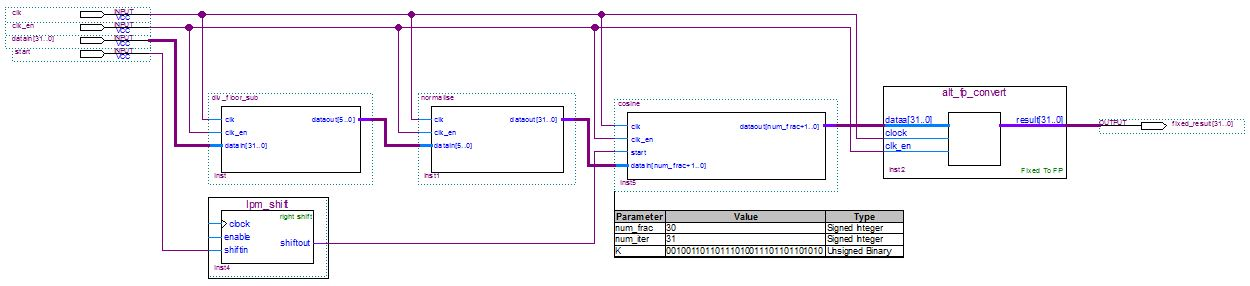
\includegraphics[width = 0.99\textwidth]{task7_bdf}
    \caption{Implementation of cordic algorithm on quartus}
    \label{fig:task7_bdf_1}
\end{figure}

The latency of the design is presented in table \ref{tab:task7_design_latency}. The cordic block has a latency of $39$ cycles. This is quite high and can be significantly improved. This will be considered in section \ref{sec:task8}.

\begin{table}[H]
  \centering
    \begin{tabular}{|c|c|}
    \hline
    \multicolumn{2}{|c|}{\textbf{Task 7 Design Latency}} \\
    \hline
    \textbf{Module} & \textbf{Latency (clock cycles)} \\
    \hline
    {\tt div\_floor\_sub} & 1 \\
    \hline
    {\tt ROM}   & 1 \\
    \hline
    {\tt cosine} & 31 \\
    \hline
    {\tt ALTFP\_CONVERT} & 6 \\
    \hline
    TOTAL & 39 \\
    \hline
    \end{tabular} 
    \caption{Latency of design for task 7}
    \label{tab:task7_design_latency}
\end{table}%

\newpage
\subsection{Overall Design for Task 7}\label{sec:task7_overall}
The design proposed in section \ref{sec:cordic_design} computes the cosine in custom hardware. This design is incorporated with adders, multipliers and shift registers such that it is capable of evaluating the entire complex expression in hardware. The design is shown in figure \ref{fig:task7_bdf_2}.

\begin{figure}[H]
    \centering
    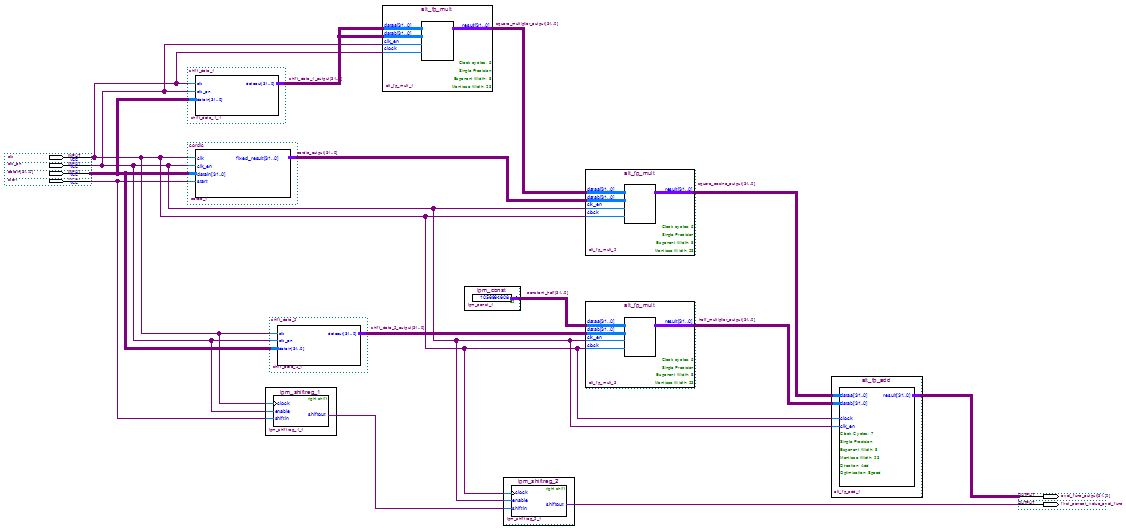
\includegraphics[width = 0.99\textwidth]{task7_bdf_2}
    \caption{Mapping entire complex expression to hardware}
    \label{fig:task7_bdf_2}
\end{figure}

Like the cordic block defined in section \ref{sec:cordic_design}, the overall design is only capable of dealing with 1 input at a time. \textbf{The overall design has a latency of 48 clock cycles.} In addition, the design is only capable of performing 1 operation. As such, a select signal is not present. The amount of resources used are listed in table \ref{tab:task7_resources}.


\begin{table}[H]
  \centering
    \begin{tabular}{|c|c|c|}
    \hline
    \multicolumn{2}{|c|}{\textbf{Hardware Description}} & \textbf{FPGA Resources} \\
    \hline
    Cache Size & 32KB  & \multirow{6}{*}{36.79\%} \\
\cline{1-2}    On-Chip Memory & 0KB   &  \\
\cline{1-2}    Logic Elements & 6,365/15,408 (41\%) &  \\
\cline{1-2}    Memory Bits & 291,885 / 516,096 ( 57\% ) &  \\
\cline{1-2}    PLLs  & 1 / 4 ( 25 \% ) &  \\
\cline{1-2}    Embedded Multiplier 9-bit Elements & 14 / 112 ( 12.5 \% ) &  \\
    \hline
    \end{tabular}%
  \caption{Resource usage for task 7}
  \label{tab:task7_resources}%
\end{table}%

\newpage
\subsection{Results for Task 7}\label{sec:task7_results}
\subsubsection{Evaluation of Function on NIOS II Processor}

The design presented in section \ref{sec:task7_overall} is tested with the function {\tt sumVector\_COMPLEX\_EXPRESSION} presented in listing \ref{lst:task7_c_code}.

\begin{listing}[H]
\begin{minted}[fontsize=\scriptsize,linenos]{C}
// function that utilises custom hardware to evaluate custom instruction
float sumVector_COMPLEX_EXPRESSION(float x[], int M)
{
	int i;
	
	// variable to hold final sum
	float running_sum = 0;
	
	for(i=0; i<M; i++){
        // call custom instruction with just 1 input
        // value returned by function is added to the running
        running_sum += ALT_CI_COMPLEX_EXPRESSION_0(x[i]);
	}
	
	// return the value of running_sum
	return running_sum;
}
\end{minted}
\caption{{\tt sumVector\_COMPLEX\_EXPRESSION}} 
\label{lst:task7_c_code}
\end{listing}


\subsubsection{Comparison of Latency}
The system is tested and results are presented in table \ref{tab:task7_latency_1}.

\begin{table}[H]
  \centering
    \begin{tabular}{|c|c|c|c|c|}
    \hline
    \textbf{N} & \textbf{Step} & \textbf{Task 5 (ticks)} & \textbf{Task 6 (ticks)} & \textbf{Task 7 (ticks)} \\
    \hline
    52    & 5     & 19    & 16    & 1 \\
    \hline
    511   & 0.5   & 185   & 164   & 5 \\
    \hline
    2551  & 0.1   & 927   & 820   & 21 \\
    \hline
    25501 & 0.01  & 9259  & 8182  & 209 \\
    \hline
    255001 & 0.001 & 92801 & 82010 & 2090 \\
    \hline
    \end{tabular}%
  \caption{Comparison of latency improvement }
  \label{tab:task7_latency_1}%
\end{table}%

\textbf{The improvement in latency is significant. Note that in both task 5 and task 7, floating-point addition is performed through software emulation.} As discussed in \ref{sec:compare_latency_6}, the main reason that the improvement in latency from task 5 to task 6 is not very significant is due to the fact that floating point operations are not the most computationally expensive step in the evaluation of the complex expression. \textbf{The very large drop in latency once the cosine is evaluated in custom hardware suggests that computing trigonometric functions through software emulation using the {\tt math.h} library is very costly. In addition, the number of custom instruction calls per iteration of the {\tt for} loop has be dramatically reduced; for task 6, the custom instruction was called 4 times per iteration whereas for task 7 the custom instruction is called just once.}\\ 

\subsubsection{Comparison of Accuracy}

The accuracy of the baseline system is studied. The results are presented in table \ref{tab:task7_accuracy}.

% Table generated by Excel2LaTeX from sheet 'Sheet6'
\begin{table}[H]
  \centering
    \begin{tabular}{|c|c|c|c|c|}
    \hline
    \multirow{2}[4]{*}{\textbf{N}} & \multirow{2}[4]{*}{\textbf{Step}} & \multicolumn{3}{c|}{\textbf{Error From Reference}} \\
\cline{3-5}          &       & \textbf{Task 5} & \textbf{Task 6} & \textbf{Task 7} \\
    \hline
    52    & 5     & -0.003 & -0.007 & -0.003 \\
    \hline
    511   & 0.5   & 0.081 & 0.093 & 0.062 \\
    \hline
    2551  & 0.1   & -1.141 & -0.875 & -1.391 \\
    \hline
    25501 & 0.01  & 14.945 & 11.945 & 11.945 \\
    \hline
    255001 & 0.001 & -202.600 & -214.600 & -154.600 \\
    \hline
    \end{tabular}%
  \caption{Comparison of accuracy}
  \label{tab:task7_accuracy}%
\end{table}%

\textbf{The results obtained from task 7 are closer to the reference value generated in MATLAB. This is exactly as expected.} The baseline design performs 30 iterative steps in the computation of the cosine. Accuracy up to $30^{th}$ bit is guaranteed since the cordic algorithm is a bit-by-bit algorithm. \textbf{It is not clear how many bits the {\tt math.h} library utilises in intermediate computations however, single-precision floating point numbers only possess $23$ mantissa bits and thus the computation is expected to be less accurate. }

\subsection{Final Comments}

\textbf{The design presented in section \ref{sec:task7_overall} will be used as a baseline for comparison.} As mentioned above, the design is only capable of dealing with 1 input and observing line 12 of listing \ref{lst:task7_c_code}, it is clear that the floating-point addition required to keep track of the running sum is performed through software emulation rather than through dedicated floating-point arithmetic units. Moreover, the fixed-point number system and the number of iterations for the cordic algorithm were arbitrarily chosen. There are significant improvements that can be made to the design and these will be discussed in section \ref{sec:task8}.

%%%%%%%%%%%%%%%%%%%%%%%%%%%%%%%%%%%%%%%%%%%%%%%%%%%%%%%%%%%%%%%%%%%%%%%%%%%%%%%%%%%%%%%%%%%%%%%%%%%%%%%%%%%%%%%%%%%%%%%%%%%%%%%%%%%%%%%%%%%%%%%%%%%%%%%%%%%%%%%%%%%%%%%%%%%%%%%%%%%%%%%%%%%%%%%%%%%%%%%%%%%%%%%%%%%%%%%%%%%%%%%%%%%%%%%%%%%%%%%%%%%%%%%%%%%%%%%%%%%%%%%%%%%%%
\newpage
\section{Task 8}\label{sec:task8}

\subsection{Improved Design}

In this section, modifications to the design presented in \ref{sec:task7_overall} will be considered. \textbf{The design that was tested in section \ref{sec:task7_results} is a very naive implementation. It did not abide by the design considerations that were set out in section \ref{sec:design_considerations}.} Firstly, it is desirable to map all floating-point arithmetic operations to hardware. The previous design did not provide support for floating point addition. Secondly, the extended custom instruction is capable of taking two inputs namely, {\tt dataa} and {\tt datab}. It is possible to use both these inputs to speed up the evaluation of the custom instruction. This was initially proposed in section \ref{sec:final_design}. Using the cordic algorithm, the evaluation of the cosine has now been mapped to hardware and so it is possible to evaluate 2 instructions at once.\\

The design in section \ref{sec:task7_overall} requires two main changes if it is to be optimised. They are:
\begin{itemize}
    \item Custom hardware should be included to perform floating-point addition. 
    \item The custom instruction should take in 2 data points. It should evaluate the complex expression for both inputs and return their sum. 
\end{itemize}

Support for floating point addition is provided using the Altera IP block {\tt ALTFP\_ADD\_SUB}. A multiplexer similar to that used in section \ref{sec:implemented_design} is needed to generate the \textbf{\textit{done}} signal. Since the custom hardware performs two operations, a select signal, \textbf{\textit{sel}} is added. The operations corresponding to the select signal are defined in table \ref{tab:task8_select}.

\begin{table}[H]
  \centering
    \begin{tabular}{|c|c|}
    \hline
    \multicolumn{2}{|c|}{\textbf{Extended Custom Instruction}}\\
    \hline
    \textbf{sel} & \textbf{Operation Performed} \\
    \hline
    0    & Evaluation of Complex Expression \\
    \hline
    1    & Addition \\
    \hline
    \end{tabular}%
  \caption{Operations corresponding to select signal for task 8}
  \label{tab:task8_select}%
\end{table}%

In addition, a shift register has been added to the design to ensure that two elements of the input vector can be processed at once. The shift register stalls one input, namely {\tt datab}, such that both inputs are sent to the cordic block sequentially. Previously, the cordic block was only able to handle 1 input however registers have been added to the cordic block so that multiple computations can be performed at once. The amount of resources used is shown in table \ref{tab:task8_resources}.

\begin{table}[H]
  \centering
    \begin{tabular}{|c|c|c|}
    \hline
    \multicolumn{2}{|c|}{\textbf{Hardware Description}} & \textbf{FPGA Resources} \\
    \hline
    Cache Size & 32KB  & \multirow{6}{*}{57.85\%} \\
\cline{1-2}    On-Chip Memory & 0KB   &  \\
\cline{1-2}    Logic Elements & 13,621/15,408 (88\%) &  \\
\cline{1-2}    Memory Bits & 291,972 / 516,096 ( 57\%) &  \\
\cline{1-2}    PLLs  & 1 / 4 ( 25 \% ) &  \\
\cline{1-2}    Embedded Multiplier 9-bit Elements & 32 / 112 ( 29\%) &  \\
    \hline
    \end{tabular}%
  \caption{Resource usage for task 8}
  \label{tab:task8_resources}%
\end{table}%

\newpage
\subsection{Results for Task 8}
\subsubsection{Evalution of Function on NIOS II Processor}
Listing \ref{lst:task8} presents the function {\tt sumVector\_COMPLEX\_EXPRESSION\_IDEAL} that is used to test the new design.

\begin{listing}[H]
\begin{minted}[fontsize=\scriptsize,linenos]{C}
// function that utilises custom hardware to evaluate custom instruction
float sumVector_COMPLEX_EXPRESSION_IDEAL(float x[], int M)
{
    int i;
    // variable to hold final sum
    float running_sum = 0;
    // check if number of elements is even
    if(N%2 == 0){
        for(i=0; i<M; i = i+2){
            // perform both evaluation of function and floating point addition in hardware
            running_sum = ALT_CI_COMPLEX_EXPRESSION_IDEAL_0(1, sum, ALT_CI_COMPLEX_EXPRESSION_IDEAL_0(0, x[i], x[(i+1)]));
        }
        
    }
    // else if number is odd
    else{
        for(i=0; i<(M-2); i = i+2){
            // perform both evaluation of function and floating point addition in hardware
            running_sum = ALT_CI_COMPLEX_EXPRESSION_IDEAL_0(1,sum,ALT_CI_COMPLEX_EXPRESSION_IDEAL_0(0,x[i],x[(i+1)]));
        }
        // add last element
        running_sum = ALT_CI_COMPLEX_EXPRESSION_IDEAL_0(1,sum,ALT_CI_COMPLEX_EXPRESSION_IDEAL_0(0,x[M-1],0));
    }
    // return the value of running_sum
    return running_sum;
}
\end{minted}
\caption{{\tt sumVector\_COMPLEX\_EXPRESSION\_IDEAL}} 
\label{lst:task8}
\end{listing}

\subsubsection{Comparison of Latency}
The updated design is tested and the results are presented in table 8.

\begin{table}[H]
  \centering
    \begin{tabular}{|c|c|c|c|c|c|}
    \hline
    \textbf{N} & \textbf{Step} & \textbf{Task 5 (ticks)} & \textbf{Task 6 (ticks)} & \textbf{Task 7 (ticks)}  & \textbf{Task 8 (ticks)} \\
    \hline
    52    & 5     & 19    & 16    & 1 & 0\\
    \hline
    511   & 0.5   & 185   & 164   & 5 & 2 \\
    \hline
    2551  & 0.1   & 927   & 820   & 21 & 7  \\
    \hline
    25501 & 0.01  & 9259  & 8182  & 209 & 74  \\
    \hline
    255001 & 0.001 & 92801 & 82010 & 2090 & 745 \\
    \hline
    \end{tabular}%
  \caption{Comparison of latency improvement for task 8}
  \label{tab:task7_latency_1}%
\end{table}%

\textbf{The results obtained are exactly as expected. Evaluating two data elements at once and performing all floating point operations in custom hardware significantly decreased the latency.}

\subsubsection{Comparison of Accuracy}
The accuracy of the updated system is studied. The results are presented in table \ref{tab:task8_accuracy}.

% Table generated by Excel2LaTeX from sheet 'Sheet6'
\begin{table}[H]
  \centering
    \begin{tabular}{|c|c|c|c|c|c|}
    \hline
    \multirow{2}[4]{*}{\textbf{N}} & \multirow{2}[4]{*}{\textbf{Step}} & \multicolumn{4}{c|}{\textbf{Error From Reference}} \\
\cline{3-6}          &       & \textbf{Task 5} & \textbf{Task 6} & \textbf{Task 7} & \textbf{Task 8} \\
    \hline
    52    & 5     & -0.003 & -0.007 & -0.003 & -0.005 \\
    \hline
    511   & 0.5   & 0.081 & 0.093 & 0.062 & -0.001 \\
    \hline
    2551  & 0.1   & -1.141 & -0.875 & -1.391 & -0.172 \\
    \hline
    25501 & 0.01  & 14.945 & 11.945 & 11.945 & 10.195 \\
    \hline
    255001 & 0.001 & -202.600 & -214.600 & -154.600 & 213.390\\
    \hline
    \end{tabular}%
  \caption{Comparison of accuracy for task 8}
  \label{tab:task8_accuracy}%
\end{table}%

The results obtained are as expected. There is a slight variation in the error obtained, however this is due to the fact that floating-point arithmetic is not commutative/dissociative; the order in which operations are performed will slightly change the final result obtained.

\subsection{Fixed-Point Number System Analysis}\label{sec:fixed_point_num_analysis}

\textbf{In this section, analysis will be conducted to determine the ideal fixed-point number system. As mentioned in section \ref{sec:normalise}, the fixed-point number system was chosen such that the word would be 32 bits long.} By determining the range of the real numbers that the fixed-point number system was required to represent, it was noted that only 2 integer bits are required. The other 30 bits were used as fractional bits.\\ 

Following this, it was observed that the precision of the results obtained was actually better than the precision of using the {\tt math.h} library on the NIOS II processor. This was expected. \textbf{The {\tt math.h} library operates on single precision floating-point numbers that only contain $23$ mantissa bits and thus the implementation discussed in section \ref{sec:normalise} that uses $30$ fractional bits is expected to yield more accurate results.}\\

While considering the ideal fixed-point number system, it is key to identify the two variable parameters.
\begin{enumerate}
    \item \textbf{The number of iterations of the cordic algorithm}: The number of iterations will determine the latency of the cordic block implemented in section \ref{sec:cordic_design}. Although other modules within the cordic block contribute to the latency, the main delay comes from evaluating the cosine. The greater the number of iterations, the greater the latency.
    \item \textbf{The number of fractional bits in the fixed-point number}: The number of fractional bits determines the amount of resources the system will utilise.  
\end{enumerate}

\textbf{Next, it is important to note that the maximum number of iterations is determined by the number of fractional bits.} At small angles, the approximation that $arctan(\alpha) \approx \alpha$ becomes valid. As such, if the fixed-point number has $30$ fractional bits, the smallest elementary angle that can be represented is $tan(2^{-30}) \approx 2^{-30}$. Beyond the $31^{st}$ iteration of the cordic algorithm, the elementary angle that has to be subtracted/added to the reference angle cannot be represented by the fixed-point number system. \textbf{As such, the number of iterations is upper bounded by the number of fractional bits.}\\

\textbf{The converse is not true. The fixed-point number system can have a greater number of fractional bits than the number of iterations of the cordic algorithm.} The merits of having more fractional bits than the number of iterations are unclear and thus testing is performed with multiple fixed-point number systems.\\ 

To test the precision of the different fixed-point number systems, the test bench presented in appendix \ref{app:test_bench} was used. Using the test bench, multiple fixed-point number representations were tested. Three combinations produced results that should be analysed carefully. The combinations are:
\begin{enumerate}
    \item 30 Fractional bits, 31 Iterations
    \item 23 Fractional bits, 24 Iterations
    \item 30 Fractional bits, 24 Iterations
\end{enumerate}

\textbf{The implementation used in section \ref{sec:cordic_design} that uses 30 fractional bits and 31 iterations is used as the baseline case. Figure \ref{fig:fixed_point_comparison} shows the error that the other two number representations incurred with respect to the baseline case.} Note that the error that is graphed is the error incurred in the evaluation of the cosine for a set of input values. The error incurred in the cosine is very strongly correlated to the error incurred in the overall result.

\begin{figure}[H]
    \centering
    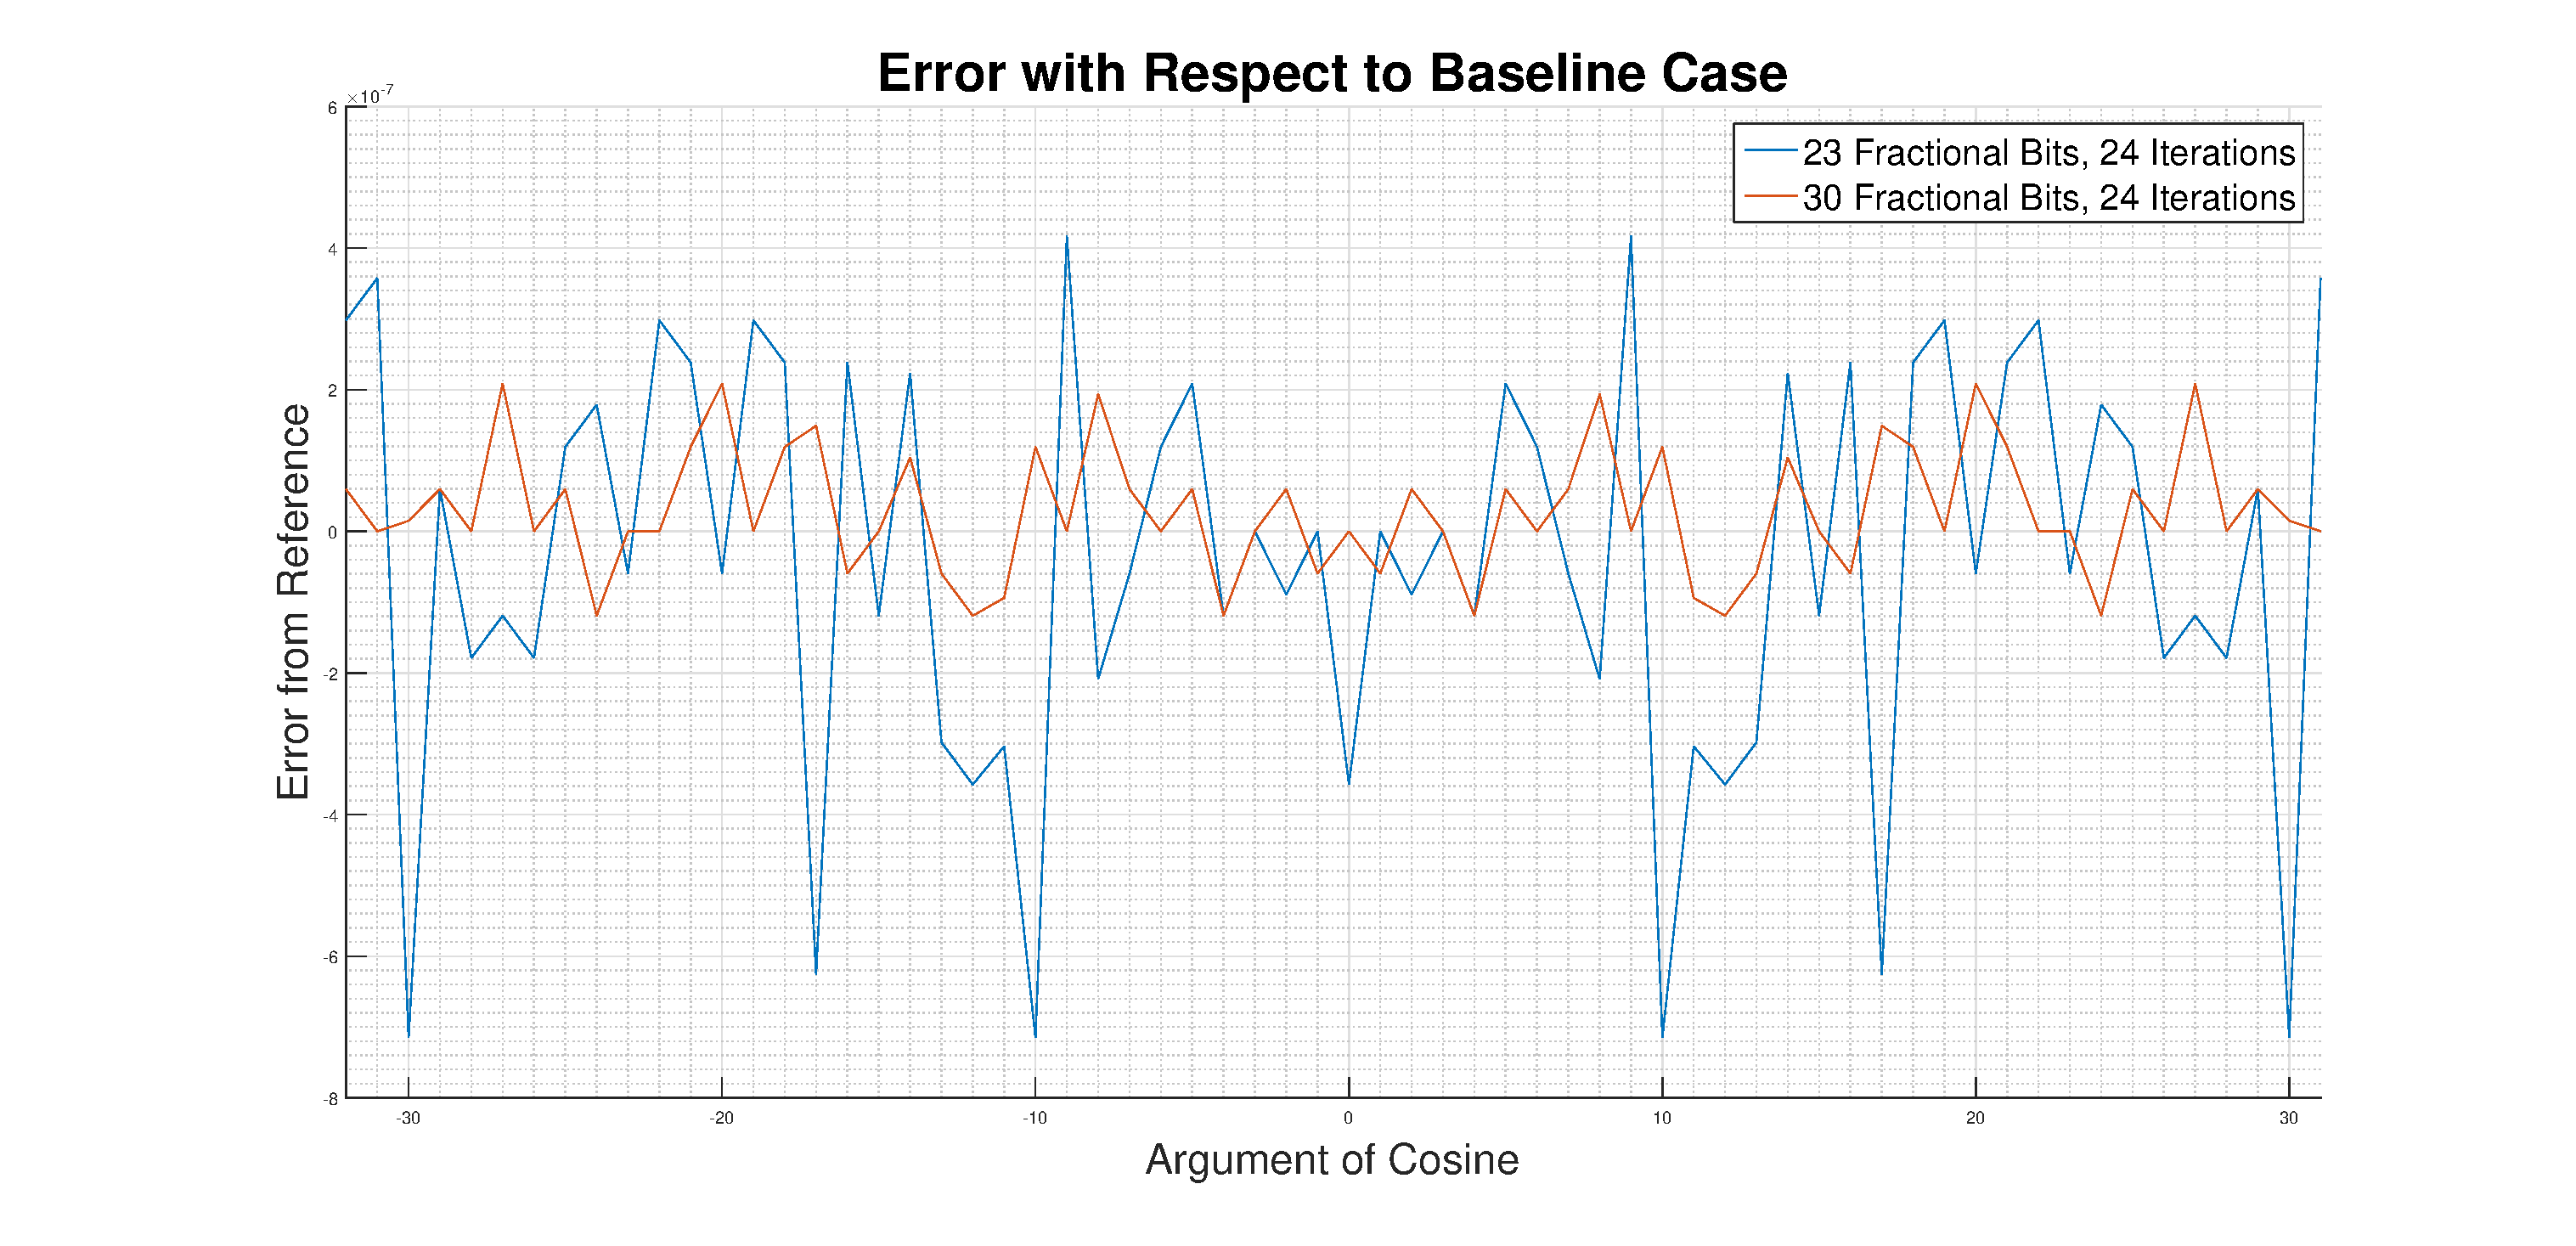
\includegraphics[width = 0.9\textwidth]{fixed_point_comparison}
    \caption{Error incurred for different fixed-point number representations}
    \label{fig:fixed_point_comparison}
\end{figure}

From the results obtained, two things are clear.
\begin{enumerate}
    \item \textbf{The magnitude of the error incurred at each evaluation of the cosine using only 24 iterations of the cordic algorithm is very small.} The maximum error incurred in any 1 calculation of the cosine is $7.15e-07$. Even if this error was to be incurred for each cosine that is evaluated, the error in the final result will be approximately $4000$. In terms of percentage error, this equates to incurring a $0.01\%$ error.
    \item \textbf{Secondly, it is clear that precision can be improved if the number of fractional bits is increased.} Initially, this result seems unexpected and thus closer inspection of the result is necessary.
\end{enumerate}


Consider a fixed-point number system that has 30 fractional bits,

\begin{align}
    cos(0) &= 1\nonumber\\
    Fixed \ Point \ Representation&: 01.\highlight{00000000000000000000000}0000000\nonumber\\\nonumber\\
    cos(30) &= 0.1542514\nonumber\\
    Fixed \ Point \ Representation&: 00.001\highlight{00111011111010000010111}1001\nonumber 
\end{align}

The highlighted bits indicate the bits that will be used to form the mantissa when the number is converted from a fixed-point representation to a floating point representation. Next consider a fixed-point number system that has only 23 fractional bits,

\begin{align}
    cos(0) &= 1\nonumber\\
    Fixed \ Point \ Representation&: 01.\highlight{00000000000000000000000}\nonumber\\\nonumber\\
    cos(30) &= 0.1542514\nonumber\\
    Fixed \ Point \ Representation&: 00.001\highlight{00111011111010000010}\highlightred{000}\nonumber\\
\end{align}

The bits highlighted in red represents the bits that need to be padded to the result to convert the fixed-point number into a floating-point number. It is clear that the number of fractional bits affects the accuracy of result. \textbf{Another interesting observation is that there is a greater error incurred for inputs that produce small results. The smaller the result, the greater the number of bits that need to be padded and the greater the error that will be incurred.} Using only 24 iterations but 30 fractional bits is balanced trade off between speed and resources.\\

\newpage
Lastly, the 3 fixed point number systems are tested on the NIOS II processor and the results obtained are presented in table \ref{tab:fixed_point_analysis}. \textbf{The error presented is with respect to the MATLAB reference value.}

\begin{table}[H]
  \centering
    \begin{tabular}{|c|c|c|c|c|c|c|c|}
    \hline
    \multirow{4}{*}{\textbf{N}} & \multirow{4}{*}{\textbf{Step}} & \multicolumn{2}{c|}{\textbf{30 Fractional Bits}} & \multicolumn{2}{c|}{\textbf{23 Fractional Bits}} & \multicolumn{2}{c|}{\textbf{30 Fractional Bits}} \\
\cline{3-8}          &       & \multicolumn{2}{c|}{\textbf{31 Iterations}} & \multicolumn{2}{c|}{\textbf{24 Iterations}} & \multicolumn{2}{c|}{\textbf{ 24 Iterations}} \\
\cline{3-8}          &       & \textbf{Time} & \textbf{Error from } & \textbf{Time} & \textbf{Error from} & \textbf{Time} & \textbf{Error from} \\
          &       & \textbf{ (ticks)} & \textbf{Reference} & \textbf{ (ticks)} & \textbf{Reference} & \textbf{ (ticks)} & \textbf{Reference}\\
    \hline
    52    & 5     & 0     & 0.005 & 0     &  0.044 & 0     & 0.013 \\
    \hline
    511   & 0.5   & 2     & -0.001 & 1     & 0.687 & 2    & 0.085 \\
    \hline
    2551  & 0.1   & 7     & -0.172 & 7     & 3.078 & 7     & 0.570 \\
    \hline
    25501 & 0.01  & 74    & 10.195 & 72    & 43.070 & 72    & 13.195 \\
    \hline
    255001 & 0.001 & 745   & 213.390 & 726   & -389.390 & 727   & 161.390 \\
    \hline
    \end{tabular}%
  \caption{Fixed-Point Number System Analysis}
  \label{tab:fixed_point_analysis}%
\end{table}%


\textbf{The results corroborate the findings obtained through simulation.}
\begin{itemize}
    \item \textbf{Reducing the number of iterations speeds up the  evaluation of the complex expression. If the number of iterations is kept constant, but the number of fractional bits is increased, the latency of the system does not increase. The latency depends solely on the number of iterations of the cordic algorithm.}
    \item \textbf{Likewise increasing the number of fractional bits without changing the number of iterations reduces the error.}
\end{itemize}

A more detailed analysis for the ideal fixed point number representation can be performed, however is skipped due to the lack of time.\\ 

\subsection{Final Design}

\textbf{\textit{The final implementation has 30 fractional bits in the fixed-point number and will perform 24 iterations of the cordic algorithm. The custom instruction takes 2 elements as inputs, evalutes the complex expression of each input sequentially; a pipeline is in place and thus the delay between the computations is just 1 clock cycle. It returns the sum of the two results. The custom instruction is also capable of performing floating point addition. The overall system has a latency 727 ticks and a percentage error of 4.359e-4\%. It uses 82\% of the logic elements, 57\% of the memory bits and 29\% of the embedded multipliers available; this adds up to using 56\% of the FPGA resources.}} 

\subsection{Final Comments}

The final design presented in section \ref{sec:fixed_point_num_analysis} can still be improved. Presented below is a discussion of what further improvements would entail.\\ 

Firstly, there are two approaches to evaluating 2 elements of the input vector within 1 call of the custom instruction. \textbf{The data points can either be evaluated sequentially or they can be evaluated in parallel.} Design consideration 4 states that the amount of resources should be minimised, however if resources can be traded for a reduction in latency, then the design that reduces latency will be preferred. In section \ref{sec:task8}, the design processed the two inputs {\tt dataa} and {\tt datab} sequentially. Processing data sequentially will increase the latency, albeit not significantly. As such, the two data points could have been evaluated in parallel. Without testing, it is hard to say how sizable the impact of processing the two elements in parallel would be. By decreasing the number of iterations of the cordic algorithm from 31 to 24, 7 clock cycles, for each custom instruction call, were saved. If the instruction is called $255001$ times, the decrease in latency should be about $35$ ticks. As seen from table \ref{tab:fixed_point_analysis}, the decrease in latency was actually 19 ticks for test case 3. Saving 2 clock cycles by processing the two elements in parallel will ideally save $10$ ticks. If not for the lack of time, experimentation would have been conducted. The entire hardware presented in section \ref{sec:task7_overall} could have been duplicated and the latency analysed.\\

\textbf{Secondly, it was noted that the final design in section \ref{sec:fixed_point_num_analysis} only performed 1 iteration of the cordic algorithm in each clock cycle. This is an extremely inefficient implementation. Processing 1 iteration of the cordic algorithm using combinations logic does not take $20ns$. To reduce the latency of the design, it is preferable to use as much of each clock cycle to perform computations, i.e to minimise the slack time. The design in section \ref{sec:task7_overall} spends a large proportion of each clock cycle idle. As such, more iterations of the cordic algorithm should be performed in each clock cycle.} \\

\textbf{If all 31 iterations were performed in 1 clock cycle, the critical path of the combinatorial logic will be too long; the design will need a clock that is slower than $50Mhz$. To reduce the length of the critical path and ensure that the design works well with a $50Mhz$ clock, registers can be added to hold intermediary values. This is called pipelining. Registers are typically introduced in digital systems to break computations into smaller parts. This will reduce the critical path between combinatorial logic and increase the maximum operating frequency. In this application, the clock frequency is fixed and thus it is advisable to only break the computations into the minimum number of stages required to meet an operating frequency of $50MHz$.}\\

Lastly, a great deal of time was spent trying to configure the control signals needed for direct memory access. A 24 stage pipeline was designed and simulated on ModelSim. The proposed design worked exactly as expected; it was able to cope with data that was streamed in; the system could handle processing a new data every clock cycle. In hindsight, it was foolish to implement a 24 stage pipeline. As discussed above, by performing multiple iterations in 1 clock cycle, the number of pipeline stages could have been significantly reduced. The control signals for the Avalon Memory-Mapped Master were configured. Initial testing was done and the system was able to read the input vector directly from memory. However, once the entire system was designed and data was streamed in from memory, the results obtained were extremely inconsistent.
 
\section{Conclusion}
In conclusion, although the final design can still be further optimised, it is clear that incorporating custom hardware to perform complex equations can significantly improve the performance of a digital system.\\ 

\textbf{\textit{Throughout the Digital Systems Design coursework, both students picked up invaluable skills necessary for designing digital systems. It was thoroughly enjoyable.}}

\newpage
\appendix
\section{Test Bench used to Evaluate Fixed-Point Number Systems}\label{app:test_bench}
\begin{minted}[fontsize=\scriptsize,linenos]{Verilog}
//-------------------------------------------------------------------------------------------------
// define timescale and operating precision
`timescale 1ns/100ps

//-------------------------------------------------------------------------------------------------
// MODULE NAME: 
//      cosine_tb
//
// MODULE FUNCTION:
//      test bench to evaluate different fixed point number representations
//      works only with cosine block rather than entire system
//      cosine block is fed with inputs read from text file
//      64 inputs are tested
//      outputs are written to text file such that date can be analysed in MATLAB
//      num_frac is a parameter that defines the number of fractional bits
//      num_iter is a parameter that defines the number of iterations of the cordic algorithm
//      
module cosine_tb();


//-------------------------------------------------------------------------------------------------
// parameters for cosine_tb module
parameter num_frac = 30;
parameter num_iter = 30;
// length of K depends on the number of fractional bits
parameter K = 'b00100110110111010011101101101010;

//-------------------------------------------------------------------------------------------------
// parameters needed for file and for loop
// N_vectors defines the number of inputs that the cosine block is tested for
parameter num_inputs = 64;
reg [num_frac+1:0]  inputs_to_be_tested [num_inputs:0];

//-------------------------------------------------------------------------------------------------
// inputs to Device-Under-Test (DUT): need to be regs  
reg                 clk;
reg                 clk_en;
reg [num_frac+1:0]  datain;

//-------------------------------------------------------------------------------------------------
// outputs from DUT: need to be wire
wire  [num_frac+1:0]  dataout;

//-------------------------------------------------------------------------------------------------
// integers needed for file and for loop
integer f_input;
integer f_output;
integer i, j;

//------------------------------------------------------------------------------------------------
// instantiate DUT
// using named instantiation
cosine CFP1(.clk(clk),
            .clk_en(clk_en),
            .datain(datain),
            .fixed_result(result));

//------------------------------------------------------------------------------------------------
// create a 50MHz clock
always
    // invert clock every 10ns seconds
    #10 clk = ~clk;
  
//------------------------------------------------------------------------------------------------
// read input from file and store in vector t
initial begin

    // open input file in read mode
    f_input = $fopen("input", "r");
    
    // display that input file is being read on console
    $display($time, " << Reading Input Vector >> ");
    
    // all inputs to be tested are read into vectored named inputs_to_be_tested
    for(i = 0; i<num_inputs; i = i+1) begin
        // read input from file into vector
        $fscanf(f_input, "%b", inputs_to_be_tested[i]);
        
    end
    
    // display that all inputs to be tested have been read
    $display($time, " << Finished Reading Input Vector >> ");
    
    // close the input file
    fclose(f_input);

end

//------------------------------------------------------------------------------------------------
// initial block sends input into cordic block
initial begin 
    
    // initialise all inputs to 0 at time 0
    clk = 1'b0;
    en  = 1'b0;
    datain = 'b0;
    
    // wait 10 nanoseconds and assert clk_en
    #10
    clk_en = 1'b1;
    
    for( i = 0; i < N_vectors; i = i +1) begin
    
        // feed input
        datain = inputs_to_be_tested[i];
        
         // wait 1 clock cycle     
        #20
        
    end

end

//------------------------------------------------------------------------------------------------
// initial block reads outputs and prints to file
initial begin 
    
    // open the output file where results are to be printed
    // file opened in write mode
    // name of file depends on num_iter and num_frac
    f_output = $fopen("cordic_output_30_fractional_31_iterations.txt", "w");
    
    // initial delay: waiting for pipeline to fill up
    // delay is depended on number of iterations
    #630
    
    // after initial delay results will be ready every clock cycle
    for( j = 0; j < N_vectors; j = j +1) begin
    
        // display result on screen
        // display index of for loop as well
        $display($time, " index: %d, dataout = %b ", j-32, dataout);
        
        // write result to output file
        $fwrite(f_output, "%b\n", dataout);
        
        // wait 1 clock cycle
        #20
        
    end
    
    // close output file
    $fclose(f_output);
    
end
endmodule
\end{minted}
\captionof{listing}{Test bench used to evaluate number systems}\label{lst:test_bench}


\end{document}

